\section{Git Tortoise}
\begin{frame}[allowframebreaks]
\frametitle{Git Tortoise}
\begin{itemize}
\item \textit{Jednostavan za korištenje:}
{\setlength\itemindent{15pt}\item sve naredbe dostupne su izravno iz Windows Explorera}
{\setlength\itemindent{15pt}\item pregled statusa datoteka izravno u Windows Exploreru}
{\setlength\itemindent{15pt}\item opisni dijalozi}
{\setlength\itemindent{15pt}\item stalno se poboljšava zbog povratnih informacija korisnika}
{\setlength\itemindent{15pt}\item dopušta premještanje datoteka}
\framebreak
\item \textbf{kontekstni izbornik-} glavni način interakcije s TortoiseGit
 \item na sljedećoj slici vidite nekoliko mogućih opcija: 
 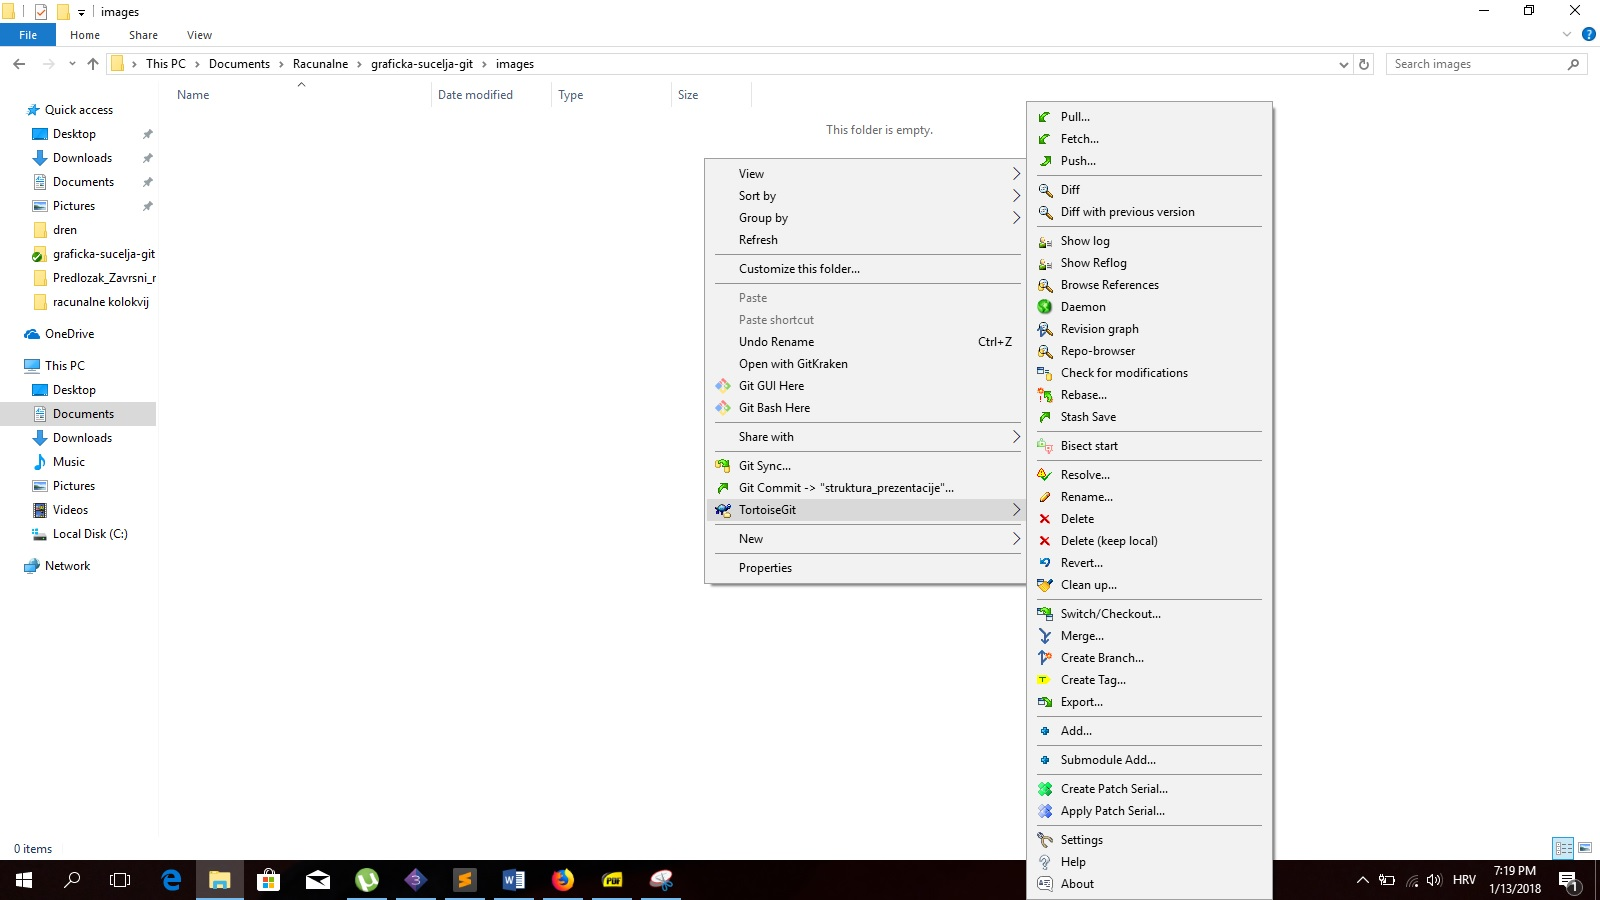
\includegraphics[width=0.8\linewidth]{images/git_tortoise.jpg}
 \framebreak
 \item \textbf{Sadrži:}
 {\setlength\itemindent{15pt}\item snažan dijaloški okvir za izvršavanje}
 {\setlength\itemindent{15pt}\item provjeru pravopisa za log poruke}
 {\setlength\itemindent{15pt}\item automatsko dovršavanje putova i ključnih riječi modificiranih datoteka}
 {\setlength\itemindent{15pt}\item oblikovanje teksta s posebnim znakovima}
 \framebreak
 \item integracija sa sustavima za praćenje problema
 \item pruža fleksibilan mehanizam za integraciju bilo kojeg web sustava za praćenje bugova
 \item zaseban ulazni okvir za unos broja issuea dodijeljenog commitu 
 \item kod prikaza log poruka, dodaje se dodatni stupac s brojem issuea (odmah možete vidjeti kojem issueu commit pripada)
 \item brojevi issuea pretvaraju se u linkovi koje otvaraju webbrowser izravno na odgovarajućem issueu
 \item opcionalno upozorenje ako se commit ne dodjeljuje broju issuea
 \framebreak
\item \textit{Korisni alati:}
 \item \textbf{TortoiseGitMerge:}
 {\setlength\itemindent{15pt}\item prikazuje promjene koje ste napravili u datotekama}
 {\setlength\itemindent{15pt}\item pomaže u rješavanju sukoba}
 {\setlength\itemindent{15pt}\item može primijeniti patchfile koje ste dobili od korisnika bez predajnog pristupa vašem spremištu}
 \item \textbf{TortoiseGitBlame:}
 {\setlength\itemindent{15pt}\item prikazuje krivnju datoteka}
 {\setlength\itemindent{15pt}\item prikazuje i zapisničke poruke za svaku liniju u datoteci}
 \item \textbf{TortoiseGitIDiff:}
 {\setlength\itemindent{15pt}\item prikazuje promjene koje ste napravili na slikovnim datotekama}
 \framebreak
 \item dostupan na mnogim jezicima
 \item stabilan
 \item klijent za kontrolu revizije Git
 \item besplatan softver, objavljen pod GNU General Public License.
 \item nudi ikonske slojeve koji upućuju na status Gitovih stabala i datoteka
 \item dolazi s TortoiseGitMerge programom za vizualnu usporedbu dviju datoteka i rješavanje sukoba
\end{itemize}
\end{frame}